Im Folgenden werden die theoretischen Grundlagen der Elektronenspinresonanz erläutert. Hierzu ist vor allem die Herleitung des magnetischen Moments in Folge des Bahndrehimpulses und des Spins sowie die Aufspaltung der Energienieveaus in einem Magnetfeld in Abhängigkeit des magnetischen Momentes wichtig.
\subsection{Magnetisches Moment -- Herleitung}
Das magnetische Moment ist das Produkt aus einem Kreisstrom und der umlaufenen Fläche. Um die Teilchenströme eines Atoms zu berechnen betrachtet man die Wellenfunktionen eines Atoms in Kugelkoordinaten $(r, \theta, \phi)$
\begin{equation}
	\psi_{\textrm{n,l,m}}(r, \theta, \phi) = \textrm{R}_{\textrm{n,l}}(r)  \, \Theta_{\textrm{ l,m}}(\theta)  \, \Phi_{\textrm{m}}(\phi) \quad .
\end{equation}
Relevant sind die Hauptquantenzahl $n \in \mathbb{N}$, die Bahndrehimpulsquantenzahl $l = \frac{k}{2}, k \in \mathbb{N}$ und die Orientierungsquantenzahl $m \in  (-l, -l+1, ..., l)$. Alle Anteile der Wellenfunktion sind normiert und es gilt
\begin{equation*}
	 \Phi_{\textrm{m}}(\phi) = \frac{1}{\sqrt{2 \pi}} \textrm{e}^{i \textrm{m} \phi}  \quad \textrm{und} \quad  \textrm{R}_{\textrm{n,l}}(r),  \Theta_{\textrm{ l,m}}(\theta) \in \mathbb{R} \quad .
\end{equation*}
Nur der azimutale Anteil der Wellenfunktion trägt zur Teilchenstromdichte~$\va{S}$ bei, da alle anderen Anteile rein reellwertig sind
\begin{equation}
	\va{S} = \frac{\hbar}{2 i \textrm{m}_0} \left( \psi^* \grad \psi - \psi \grad \psi^*  \right)
	= \frac{\hbar \textrm{R}^2 \Theta^2 \textrm{m}}{\textrm{m}_0 2 \pi r \sin{\theta}} = \va{S}_\phi \quad .
\end{equation}
Die elektrische Stromdichte~$j_\phi$ (Strom~$I$ pro Fläche~$f$) folgt aus der Teilchenstromdichte
\begin{equation}
	j_\phi = \dv{I_\phi}{f} = - \textrm{e}_0 S_\phi \quad .
\end{equation}
Mit geometrischen Überlegungen (siehe Abb. \ref{fig:geometrie}) erhält man das magnetische Moment~$\mu_z$ des Elektrons in $z$-Richtung als Produkt des Kreisstroms~$I_\phi$ und der umlaufenen Fläche~$F(\theta)$
\begin{align}
	\dd{\mu_z} &= F(\theta)  \dd{I_\phi} = \left(\pi r^2 \sin^2{\theta} \right)
 	\left(   \frac{\hbar \textrm{R}^2 \Theta^2 \textrm{m}}{\textrm{m}_0 2 \pi r \sin{\theta}}  r \dd{\theta} \dd{r} \right)  \\
 	\Rightarrow \mu_z &= \int_{0}^{\infty} \int_{0}^{\pi} F(\theta) j_\phi r \dd{\theta} \dd{r}  \\
 	&= - \frac{\textrm{e}_0 \hbar}{2 m_0} \textrm m = \mu_\textrm{B} \textrm{m} \quad .
\end{align}

\begin{figure}[h!]
	\centering
	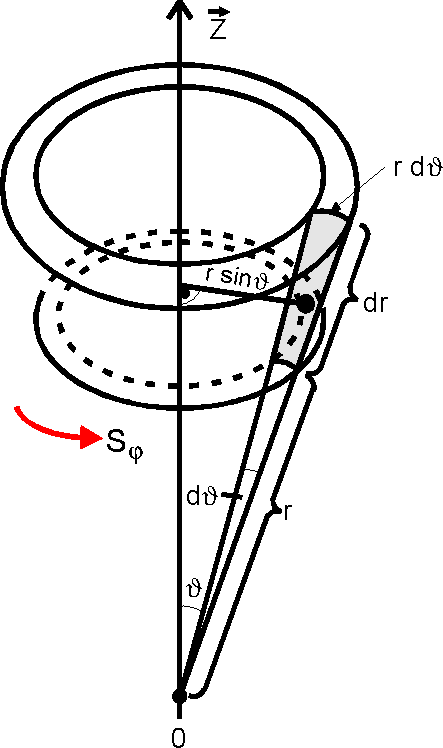
\includegraphics[width=0.3\textwidth]{Anleitung_Abb1.pdf}
	\caption[Geometrische Betrachtung]{Geometrische Betrachtung des Flächenelements $\\d{f} = r \dd{r} \dd{\theta}$  und der umlaufenen Fläche $F(\theta) = \pi r^2 \sin^2{\theta}$ \cite{V28}}
	\label{fig:geometrie}
\end{figure}


Alle auftretenden Naturkonstanten werden zum Bohrschen Magneton $\mu_\textrm{B} $ zusammengefasst, sodass leicht zu erkennen ist, dass das magnetische Moment nur noch von der Orientierungsquantenzahl abhängt
\begin{equation}
	\mu_B = \SI{9.274015 \pm 0.000003}{\joule\per\tesla} \quad .
\end{equation}
Die Herleitung berücksichtigt lediglich den Bahndrehimpuls des freien Elektrons. Der Landé-Faktor~$g$ wird eingeführt, um den Spin mit einzubeziehen und um das magnetische Moment eines gebundenen Elektrons oder ganz anderen Teilchens auszurechnen.
\begin{equation}
	\mu_z = g \mu_\textrm{B} \textrm{m}
\end{equation}
Für das Elektron (Fermion) ist $\textrm{m} = \pm \frac{1}{2}$ und die Spinkorrektur beträgt $g_S = \si{2,002}$ \cite{Lande-Faktor}.
\todo[color = red]{warum ist die nummeriereung des literaturverzeichnisses in der falschen reihenfolge?}

\clearpage

\subsection{Aufspaltung der Energieniveaus in einem Magnetfeld}

Ein magnetisches Moment $\va{M}$ in einem homogenen Magnetfeld $\va{B}$ trägt eine potentielle Energie je nach der Ausrichtung relativ zu den Magnetfeldlinien
\begin{equation}
	E_\textrm{mag} = \va{M} \cdot \va{B} \quad .
\end{equation}
Wenn das magnetische Moment parallel zu den Magnetfeldlinien ausgerichtet ist, spaltet sich die Energie in $2l+1$ mögliche Energieniveaus auf. In Abb \ref{fig:energieniveaus} ist dies für den Fall $l = 2 \Rightarrow m = (-2, -1, 0, 1, 2)$ dargestellt. Der Effekt ist auch als Zeeman-Effekt bekannt. Das zugehörige Experiment ist der Stern-Gerlach Versuch.
\\

\begin{figure}[h!]
	\centering
	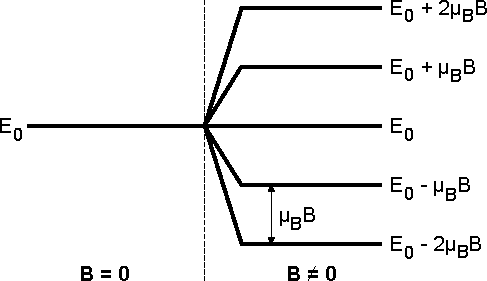
\includegraphics[width=0.5\textwidth]{Anleitung_Abb3.pdf}
	\caption[Zeeman-Effekt]{Zeeman-Effekt: Aufspaltung der Energieniveaus in einem Magnetfeld in Abhängigkeit der Orientierungsquantenzahl \cite{V28}}
	\label{fig:energieniveaus}
\end{figure}